% !TEX root = thesis_draft.tex

\section{Simulation study}

\subsection{Introduction}

While the phase locking value (PLV), circular correlation (CCorr) and
imaginary part of coherency (ImagCoh) measures have been introduced
mathematically, it can be difficult to understand what a certain inter-brain
synchrony (IBS) measure value says about the underlying data. We attempt to
shine some light on the matter using a simulation study.

We introduce a visualization that shows the relation between the phase
components of two EEG signals. For our purposes, one signal from each
participant in the dyad. We then apply this visualization method to simulated
phase data examples. The examples have been chosen such that they result in a
large range of IBS values. This allows us to see what patterns in the
phase data the IBS measures detect, and as a result what relations between the two
signals they are sensitive to (or not).

In these simulations we ignore the amplitude component. This has two reasons: it
is only actually used by the ImagCoh measure, and it would make it harder to
draw any conclusions as it would require more complex visualizations. Finally,
we explain how our approach can be used to perform a power analysis for IBS
experiments.

\subsection{Methods}

\begin{figure}[!htpb]
  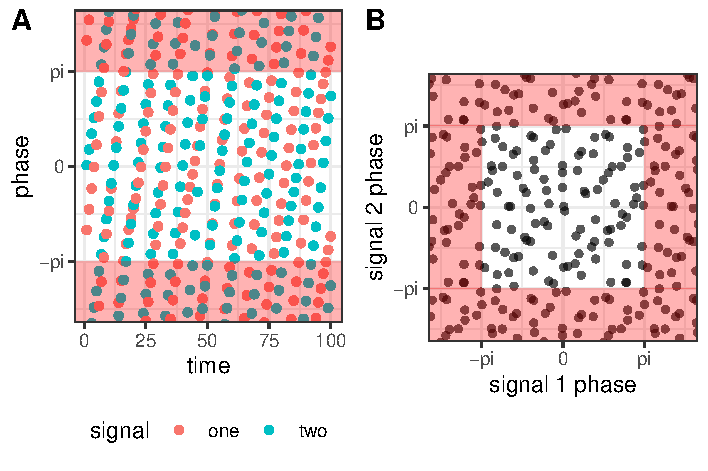
\includegraphics[width=\linewidth]{../stats/results/phases-visualization.pdf}
  \caption{Phase values of both participants in session 2, trial 1 for the Pz electrode at 11Hz. (The trial from Figure~\ref{fig:freqanalysis}.) For this trial, circular correlation = -0.01, phase locking value = 0.033 and imaginary part of coherency = 0.012 (ignoring amplitude values). Shaded areas contain repetitions of the (circular) values. (A): Phase values over time. (B): The same two signals plotted against each other, without time, to show the relation between them. This type of visualization is used throughout this simulation study.}
  \label{fig:phases-visualization}
\end{figure}

As discussed in the general introduction, comparing the relation between two
phase signals requires a space that wraps around in two dimensions. One solution
to this problem is to plot data on a torus (see Figure~\ref{fig:torus}), but
that is not practical for a two-dimensional medium like this report. It would
also result in deformed distances. Instead, we use normal plots, but visualize
the data for 1.5 periods, resulting in a repeated (and differently shaded) area
at the visualization's edges. This makes it easier to imagine the circular
repetition of the data and to spot patterns that would otherwise span the edges
of the plotting area.

We focus on a single session, trial, electrode and frequency at a time. As we
have previusly seen in Figure~\ref{fig:freqanalysis}C, this results in a
one-dimensional phase signal over time for each participant ($\phi$ and $\psi$
respectively). We reproduce these signals in
Figure~\ref{fig:phases-visualization}A, using the y-axis instead of colour to
show their values. If we then get rid of the time dimension, as all discussed
IBS measures do, we can give each phase signal its own axis in
Figure~\ref{fig:phases-visualization}B to make it easier to see the relation
between the two. The resulting plot demonstrates the primary visualization
method used in this study.

The easiest way to simulate this (empirical) phase data is to sample 100 points
from a two-dimensional uniform random distribution with a range of
$[-\pi, \pi)$. We can then calculate the IBS measures on each of these samples.
For the imaginary part of coherency measure, we use a fixed amplitude of one.
When we repeat this process 10~000 times, it results in a distribution of values
for each IBS measure created under the assumption that there is no relation
between the two signals.

While that is useful, completely random signals are unlikely to elicit the full
range of IBS values. To be able to generate signals for any measure
value, we created Algorithm~\ref{alg:optimize-measures}.

\begin{algorithm}
  \caption{Generates random phase data examples that minimize an evaluation function $f$ using a combination of global and local search.}
  \begin{algorithmic}
  \Require $f(\phi, \psi) \to \mathbb{R}$ \Comment{the evaluation function to minimize}
  \State repetitions $\gets$ the amount of global search iterations
  \State start $\gets$ the initial amount of data points in the sample (should be $\geq$ end)
  \State end $\gets$ the amount of data points in the sample after local search finishes
  \\
  \State best $\gets \infty$
  \State result $\gets [~]$
  \For{'repetitions' amount of iterations} \Comment{the global search part}
    \State $\phi, \psi \gets$ a 2D uniform random sample of length `start' and range $[-\pi, \pi)$
    \While{cur > end} \Comment{the local search part}
      \For{$i \in 1 \ldots \text{length of } \phi$}
        \State $\phi'_i, \psi_i \gets \phi, \psi$ without the $i$th values
        \State $e_i \gets f(\phi'_i, \psi'_i)$
      \EndFor
      \State $i \gets \text{argmin}(e_i)$
      \State $\phi, \psi \gets \phi'_i, \psi'_i$
    \EndWhile
    \If{$f(\phi, \psi) < \text{best}$}
      \State best $\gets f(\phi, \psi)$
      \State result $\gets [\phi~\psi]$
    \EndIf
  \EndFor
  \State\Return result
  \end{algorithmic}
  \label{alg:optimize-measures}
\end{algorithm}

Algorithm~\ref{alg:optimize-measures} finds example signals that minimize an
evaluation function $f(\phi, \psi)$. It uses a combination of global and local
search. The global search part of the process generates multiple random signals
and picks the ones that minimizes the evaluation function. The local search part
of the process optimizes each candidate before evaluation by removing a number
of `outliers' (as determined by the evaluation function), one at a time. By
varying the input parameters, it is possible to trade-off between the (unbiased,
but unlikely to cover the whole range) global search process and the (biased,
but more flexible) local search process.

We apply Algorithm~\ref{alg:optimize-measures} in two tasks.

First, we use it to generate examples that have CCorr and ImagCoh values close
to $-1, -0.75, \ldots, 0.75$ and $1$. And the same for the PLV values
$0, 0.125, \ldots, 0.875$ and $1$. To approximate values, we use an L2 loss
function as the evaluation function. E.g. to get a CCorr value of
$-0.75$ the evaluation function is
\begin{align}
  f(\phi, \psi) = \left(CCorr(\phi, \psi) - (-0.75)\right)^2,
\end{align}
where $CCorr$ is as defined in Equation~\ref{eq:ccorr}.

Secondly, to further contrain the examples and to see where the IBS measures
differ, we use evaluation functions that constrain the measures in different
ways simultaneously. For example, when minimizing the evaluation function
\begin{align}
  f(\phi, \psi) = 1 - CCorr(\phi, \psi) + |ImagCoh(\phi, \psi)| + PLV(\phi, \psi),
\end{align}
we obtain example signals with a positive CCorr value, a (close to) zero
ImagCoh value and a low PLV value. We generate example signals for all possible
constraint permutations. The $PLV$ and $ImaghCoh$ definitions are given in
Equations~\ref{eq:plv}~and~\ref{eq:imagcoh}.

\subsection{Results}

\begin{figure}[!htpb]
  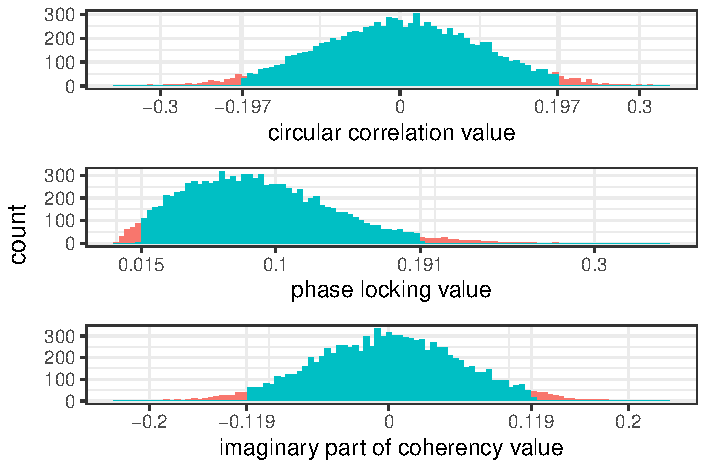
\includegraphics[width=\linewidth]{../stats/results/simulation_null.pdf}
  \caption{A histogram of inter-brain synchrony values calculated on 10~000 pairs of uniform random signals. It shows inter-brain synchrony values typical for when the underlying signals are unrelated. The central 95\% of the data is shown in blue.}
  \label{fig:simulation_null}
\end{figure}

In Figure~\ref{fig:simulation_null}, we see the distribution of IBS values
when the underlying signals are completely random. We see that the distributions
for the CCorr and ImagCoh values are symmetric and centered around their middle
value of zero. We observe a skewed distribution for the PLV measure values, most
likely because the values are all close to the minimum value the measure can
take (i.e. zero). It will be virtually impossible to distinguish an effect
that has an IBS value in the high density part of the shown distributions
from noise.

In Figure~\ref{fig:simulation_force_individually}, we see the phase components
of example signals for the whole range of CCorr, ImagCoh and PLV measure values.
Finding ImagCoh examples was harder than finding examples for the other
measures, resulting in different input parameters for
Algorithm~\ref{alg:optimize-measures} being required to cover the whole range.
These parameters can be found in Table~\ref{tab:force_individually_params}.

\begin{landscape}
  \begin{figure}
    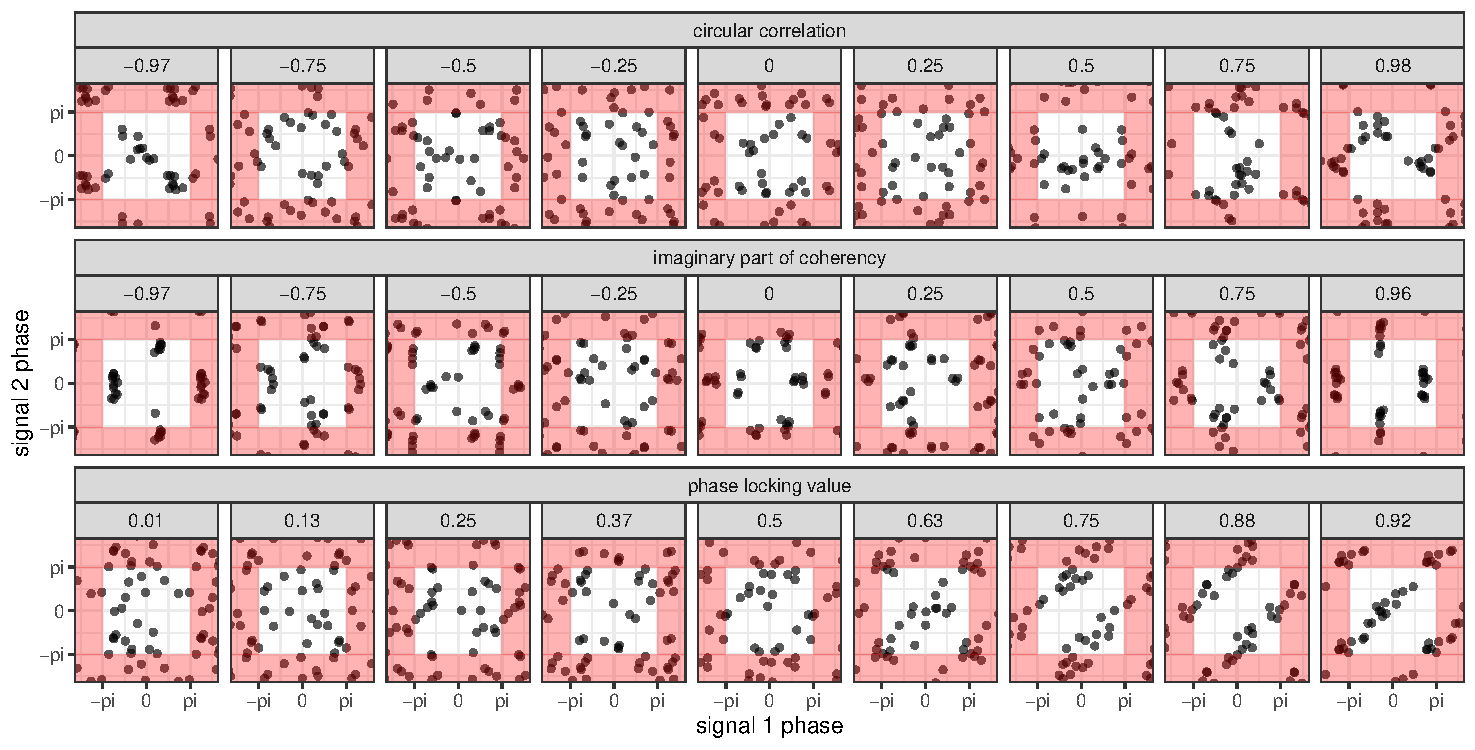
\includegraphics[width=\linewidth]{../stats/results/simulation_force_individually.pdf}
    \caption{Simulated examples for the whole range of inter-brain synchrony measure values. As in Figure~\ref{fig:phases-visualization}, shaded areas contain repetitions of the (circular) values. A high phase locking value requires a positive linear relation between signals. For a high circular correlation or imaginary part of coherency, multiple clumps suffice. But interestingly, while the simulation finds random noise examples for PLV and CCorr values of zero, the ImagCoh is assigned a clumped example instead.}
    \label{fig:simulation_force_individually}
  \end{figure}
\end{landscape}

\begin{table}[!htbp]
  \caption{Parameter values of Algorithm~\ref{alg:optimize-measures} used to generate Figure~\ref{fig:simulation_force_individually}.}
  \label{tab:force_individually_params}
  \begin{tabular}{l r r}
    \hline
    Parameter   & circular correlation \& phase locking value & imaginary part of coherency\\\hline
    repetitions &      1000 &          20\\
    start       &        40 &         200\\
    end         & (/2 =) 20 &  (/10 =) 20\\\hline
  \end{tabular}
\end{table}

The examples show a few clear trends. First of all, an increase in PLV seems to
lead to a more positive and linear relation between the phase components of the
example signals. For the other measures, higher (and lower) IBS values seem
to lead to the formation of clumps, i.e. patterns where a lot of the phase
components are approximately constant. Surprisingly, while the other measures
seem to converge on a (at first glance) random noise example for IBS values
of zero, which is in line with our findings in Figure~\ref{fig:simulation_null},
this is not the case for the ImagCoh measure. There, the
central example is clumped just like the examples at the tails.

To see whether these examples are typical or just the first configuration
Algorithm~\ref{alg:optimize-measures} finds, we further constrain the examples
by forcing them into configurations that contrast the IBS measure values.
Figure~\ref{fig:simulation_local_search} shows these examples. As this
optimization problem is harder, an optimal solution is not always found. Because
of that, the size of the error is shown as well, which is at the same scale as
the IBS values themselves. While the total error occasionally surpasses
0.5, the error is in practise divided up among measures. So while the examples
might not match the target IBS values exactly, they are never so far off as
to become misleading.

To generate Figure~\ref{fig:simulation_local_search}, 100 global search
repetitions were used. The local search started with 100 samples, and reduced
that to 20 samples.

\begin{landscape}
  \begin{figure}
    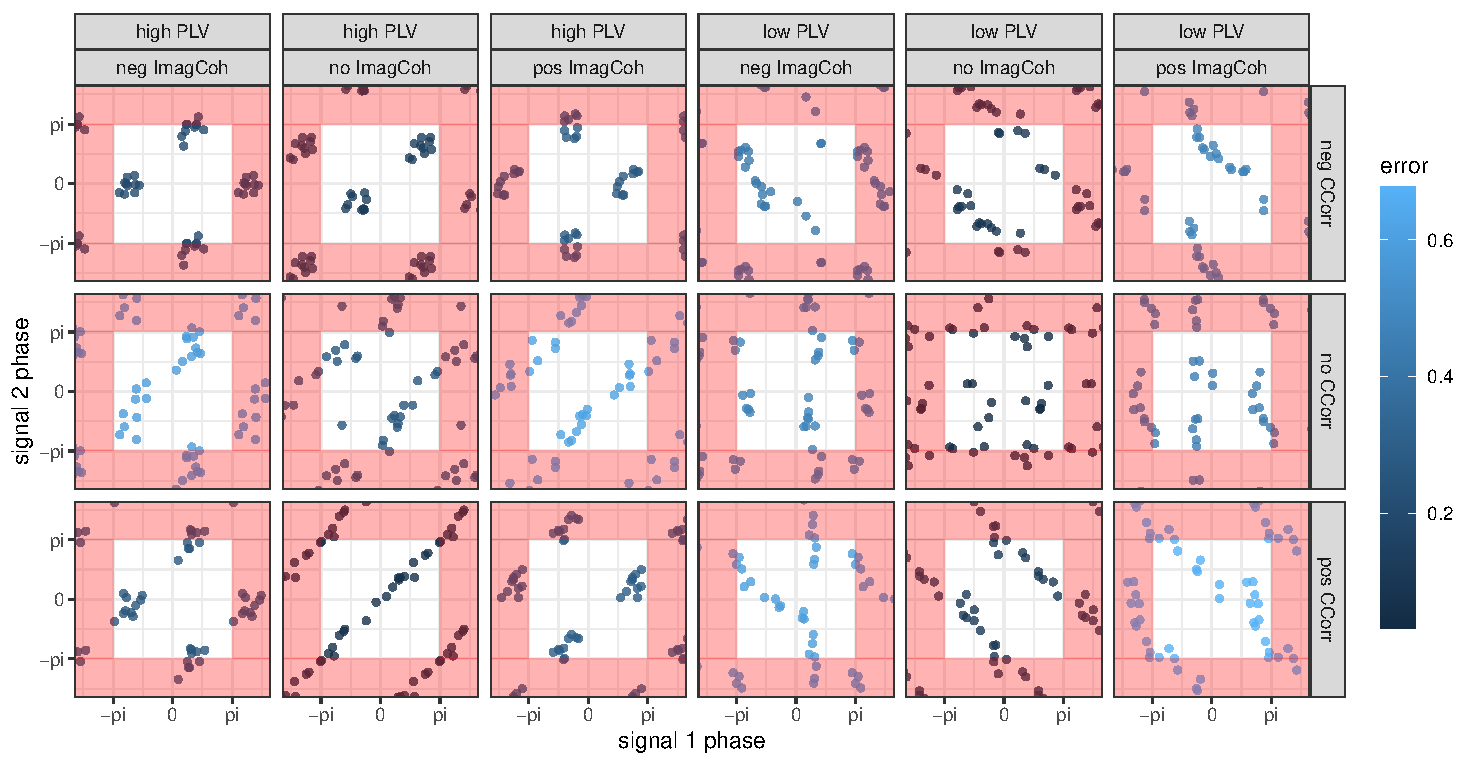
\includegraphics[width=\linewidth]{../stats/results/simulation_local_search.pdf}
    \caption{Simulated examples that minimize (low phase locking value, negative imaginary part of coherency, negative circular correlation), maximize (high PLV, positive ImagCoh, positive CCorr) or zero out (no CCorr, no ImagCoh) IBS values simultaneuously. Light blue dots indicate the example is not perfect (fulfilling the ImagCoh requirement is often most difficult), while black dots indicate all constraints were met perfectly.}
    \label{fig:simulation_local_search}
  \end{figure}
\end{landscape}

We see that PLV is not sensitive to negative linear trends (as opposed to
positive ones) at all. This is exploited in the right side of
Figure~\ref{fig:simulation_local_search}, as depending on the exact
configuration the CCorr and ImagCoh measures
are sensitive to negative trends. We further see confirmation that the imaginary
part of coherency can reach a value of zero just fine with an (apparently)
random example (the `low PLV, no ImagCoh, no CCorr' condition). Also, it is
interesting to point out that the ImagCoh is sensitive to
the phase components of signals being constant in one dimension but not in the
other, contrary to the CCorr. (See e.g. the `low PLV, no CCorr'
conditions with negative or positive ImagCoh values).
Next, it is worth noting that a configuration with a seemingly negative trend
(`low PLV, no ImagCoh, pos CCorr') results in a positive CCorr
value. Finally, to the eye immediately apparent trends are not always picked up
on by the ImagCoh measure. (E.g. the two `pos CCorr, no ImagCoh' conditions.)

\subsection{Discussion}

The lack of response of the PLV measure to a clear negative relation between the
phase components of the input signals is not unexpected, as it only reports
whether the phases are directly coupled, not if one of them can be used to
predict the other \parencite{burgess_interpretation_2013}. But it is a downside,
as you would most likely want to detect such effects in IBS experiments.

Similarly, we saw that the ImagCoh measure failed to
sometimes detect trends. That might be because it is designed not to detect
signals that are perfectly in phase, as a way to (originally) prevent spurious
effects due to volume conduction \parencite{nolte_identifying_2004}. But these
simulations suggest that the cost of that might be too high. On the other hand,
it is important to keep in mind that these simulations are not a level playing
field for the ImagCoh measure: amplitude components of the
signal on which it is normally dependent are held constant.

In the end, the CCorr values seem the least surprising
given the studied examples, although the direction of any relations (i.e.
whether the correlation coefficient is positive or negative) should probably not
be relied on.

\subsubsection{Power analysis for inter-brain synchrony experiments}

Taking a step back, it is worth pointing out that
Algorithm~\ref{alg:optimize-measures} is a very flexible method to generate
phase component data for a target IBS value. It could potentially be used to
perform an up-front power analysis for a test in an IBS experiment. The steps
would be as follows:

\begin{enumerate}
  \item Choose a target effect size. That is, what IBS value would you
  expect your experiment to find? The simulations in this section give you some
  guidance on what would be reasonable values, but ideally the target value
  would be decided based on what other similar studies found.
  \item For a range of sample sizes, repeatedly simulate the outcome of your
  test using the Monte Carlo method
  \parencite[p.~150 gives a nice introduction]{cohen_empirical_1995} as
  follows:
  \begin{enumerate}
    \item Use Algorithm~\ref{alg:optimize-measures} to generate fake trials
    for your IBS value of choice. By varying the trade-off between global- and
    local search part of the algorithm, you have some control over the variation
    around your target IBS value. Ideally, you would again use this to match
    the variation found in other similar studies.
    \item Perform your test on the simulated data, recording the outcome.
  \end{enumerate}
  \item Use the collected outcomes to estimate the power of your test for each
  sample size.
\end{enumerate}

A downside of this method, and in fact of this simulation study in general, is
that the local search part of Algorithm~\ref{alg:optimize-measures} introduces
a bias due to the way it removes outliers. After all, removing them one at a
time is just one of many possible approaches. While the results seem reasonable
looking at the graphs, it could be that some examples we observe are in fact
not typical but artifacts of the process used to generate them. This could
for example perhaps explain the clumps in the ImagCoh plot
in the very middle of Figure~\ref{fig:simulation_force_individually}.
